\documentclass[tikz,border=2pt]{standalone}
\usepackage{amsmath,amssymb}
\usepackage{tikz}
\usetikzlibrary{arrows.meta}

\begin{document}
% An Euler tour on the bow-tie network: a closed walk using every edge exactly once,
% A-B-C-A-D-E-A; the vertex A is visited twice, which is allowed.
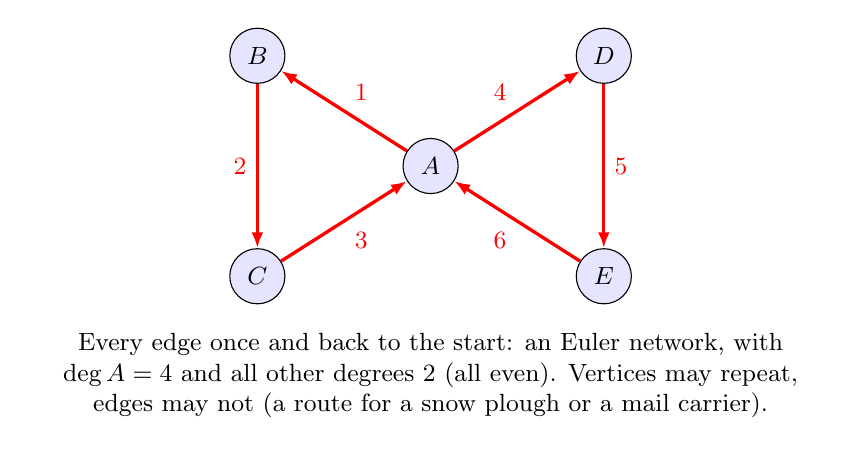
\begin{tikzpicture}[every node/.style={font=\small}, >={Latex[length=2mm]}, v/.style={draw, circle, fill=blue!10, minimum size=7mm, inner sep=0pt}]
	\node[v] (A) at (0,0) {$A$};
	\node[v] (B) at (-2.2,1.4) {$B$};
	\node[v] (C) at (-2.2,-1.4) {$C$};
	\node[v] (D) at (2.2,1.4) {$D$};
	\node[v] (E) at (2.2,-1.4) {$E$};
	\draw[red, very thick, ->] (A) -- (B) node[midway, above right] {1};
	\draw[red, very thick, ->] (B) -- (C) node[midway, left] {2};
	\draw[red, very thick, ->] (C) -- (A) node[midway, below right] {3};
	\draw[red, very thick, ->] (A) -- (D) node[midway, above left] {4};
	\draw[red, very thick, ->] (D) -- (E) node[midway, right] {5};
	\draw[red, very thick, ->] (E) -- (A) node[midway, below left] {6};
	\node[anchor=north, align=flush center, text width=10cm] at (0,-2.0) {Every edge once and back to the start: an Euler network, with $\deg A=4$ and all other degrees $2$ (all even). Vertices may repeat, edges may not (a route for a snow plough or a mail carrier).};
\end{tikzpicture}
\end{document}
